\documentclass[hidelinks,12pt]{article}
\usepackage[left=0.25cm,top=1cm,right=0.25cm,bottom=1cm]{geometry}
%\usepackage[landscape]{geometry}
\textwidth = 20cm
\hoffset = -1cm
\usepackage[utf8]{inputenc}
\usepackage[spanish,es-tabla, es-lcroman]{babel}
\usepackage[autostyle,spanish=mexican]{csquotes}
\usepackage[tbtags]{amsmath}
\usepackage{nccmath}
\usepackage{amsthm}
\usepackage{amssymb}
\usepackage{mathrsfs}
\usepackage{graphicx}
\usepackage{subfig}
\usepackage{caption}
%\usepackage{subcaption}
\usepackage{standalone}
\usepackage[outdir=./Imagenes/]{epstopdf}
\usepackage{siunitx}
\usepackage{physics}
\usepackage{color}
\usepackage{float}
\usepackage{hyperref}
\usepackage{multicol}
\usepackage{multirow}
%\usepackage{milista}
\usepackage{anyfontsize}
\usepackage{anysize}
%\usepackage{enumerate}
\usepackage[shortlabels]{enumitem}
\usepackage{capt-of}
\usepackage{bm}
\usepackage{mdframed}
\usepackage{relsize}
\usepackage{placeins}
\usepackage{empheq}
\usepackage{cancel}
\usepackage{pdfpages}
\usepackage{wrapfig}
\usepackage[flushleft]{threeparttable}
\usepackage{makecell}
\usepackage{fancyhdr}
\usepackage{tikz}
\usepackage{bigints}
\usepackage{menukeys}
\usepackage{tcolorbox}
\tcbuselibrary{breakable}
\usepackage{scalerel}
\usepackage{pgfplots}
\usepackage{pdflscape}
\pgfplotsset{compat=1.16}
\spanishdecimal{.}
\renewcommand{\baselinestretch}{1.5} 
\renewcommand\labelenumii{\theenumi.{\arabic{enumii}})}

\newcommand{\python}{\texttt{python}}
\newcommand{\textoazul}[1]{\textcolor{blue}{#1}}
\newcommand{\azulfuerte}[1]{\textcolor{blue}{\textbf{#1}}}
\newcommand{\funcionazul}[1]{\textcolor{blue}{\textbf{\texttt{#1}}}}

\newcommand{\pderivada}[1]{\ensuremath{{#1}^{\prime}}}
\newcommand{\sderivada}[1]{\ensuremath{{#1}^{\prime \prime}}}
\newcommand{\tderivada}[1]{\ensuremath{{#1}^{\prime \prime \prime}}}
\newcommand{\nderivada}[2]{\ensuremath{{#1}^{(#2)}}}


\newtheorem{defi}{{\it Definición}}[section]
\newtheorem{teo}{{\it Teorema}}[section]
\newtheorem{ejemplo}{{\it Ejemplo}}[section]
\newtheorem{propiedad}{{\it Propiedad}}[section]
\newtheorem{lema}{{\it Lema}}[section]
\newtheorem{cor}{Corolario}
\newtheorem{ejer}{Ejercicio}[section]

\newlist{milista}{enumerate}{2}
\setlist[milista,1]{label=\arabic*)}
\setlist[milista,2]{label=\arabic{milistai}.\arabic*)}
\newlength{\depthofsumsign}
\setlength{\depthofsumsign}{\depthof{$\sum$}}
\newcommand{\nsum}[1][1.4]{% only for \displaystyle
    \mathop{%
        \raisebox
            {-#1\depthofsumsign+1\depthofsumsign}
            {\scalebox
                {#1}
                {$\displaystyle\sum$}%
            }
    }
}
\def\scaleint#1{\vcenter{\hbox{\scaleto[3ex]{\displaystyle\int}{#1}}}}
\def\scaleoint#1{\vcenter{\hbox{\scaleto[3ex]{\displaystyle\oint}{#1}}}}
\def\scaleiiint#1{\vcenter{\hbox{\scaleto[3ex]{\displaystyle\iiint}{#1}}}}
\def\bs{\mkern-12mu}

\newcommand{\Cancel}[2][black]{{\color{#1}\cancel{\color{black}#2}}}


\hypersetup{
    colorlinks=true,
    linkcolor=blue,
    filecolor=magenta,      
    urlcolor=red,
    }
\usepackage{minted}
\usepackage{menukeys}

\title{\vspace{-2cm}Guía rápida para git \\ {\large Curso Física Computacional} \vspace{-3ex}}
\author{M. en C. Gustavo Contreras Mayén. \texttt{gux7avo@ciencias.unam.mx}}
\date{}

\begin{document}

\fontsize{14}{14}\selectfont
\vspace{-4cm}
\maketitle

\section{Control de versiones}

¿Qué es el \enquote{control de versiones} y por qué debería importarnos?
\\
El control de versiones es un sistema que registra los cambios que hacemos en un archivo o conjunto de archivos a lo largo del tiempo para que podamos recuperar versiones específicas más adelante.
\par
Pensemos que estamos escribiendo un trabajo final, un reporte o quizá la tesis de la carrera, y queremos conservar todas las versiones de del documento, imágenes, tablas, incluyendo códigos en algún lenguaje o programa específico (lo que sin duda deberíamo), un Sistema de Control de Versiones (Version Control System, \textbf{VCS}) es una opción muy inteligente. Ya que nos permite revertir tanto archivos como todo un proyecto a un estado anterior, comparar cambios a lo largo del tiempo, en el caso de estar elaborando un proyecto en equipo, ver quién modificó por última vez algo que podría estar causando un problema, quién introdujo un problema y cuándo, y más acciones.
\par
El uso de un VCS generalmente también significa que si por alguna razón se arruinan las cosas o se pierden archivos, podemos recuperarlos fácilmente. 

\begin{figure}[H]
    \centering
    
\includegraphics[scale=0.45]{Imagenes/meme_tesis.jpeg}
    \caption{Ejemplo de un manejo no conveniente para las versiones de la tesis.}
    \label{fig:figura_tesis}
\end{figure}

\subsection{Sistemas de control de versiones locales.}

El método de control de versiones elegido por muchas personas es copiar archivos en otro directorio (quizás un directorio con marca de tiempo, si queremos menos problemas). Este enfoque es muy común porque \textit{es muy simple}, como se muestra en la figura (\ref{fig:figura_tesis}) pero también es \textbf{increíblemente propenso a errores}: es fácil olvidar en qué directorio se encuentra y escribir accidentalmente en el archivo incorrecto o copiar archivos que no teníamos la intención de copiar.
\par
Para lidiar con este problema, un equipo de programadores desarrollaron hace mucho tiempo VCS locales que tenían una base de datos simple que mantenía todos los cambios en los archivos bajo control de revisión.
\par
Luego de continuar con el desarrollo y hacer cambios en el enfoque del manejo de un VCS, \textbf{Git} nace en año 2005, ha evolucionado y madurado para ser fácil de usar. Es increíblemente rápido, es muy eficiente con proyectos grandes y tiene un increíble sistema de bifurcación (ramas) para el desarrollo no lineal, es decir, no necesariamente los cambios se dan de manera secuencial: Capítulo 1, Capítulo 2, etc. sino que pueden ser: Capítulo 5, Capítulo 2, Bibliografía, Introducción, etc.

\section{Conceptos básicos de Git.}

Entonces, ¿qué es Git en pocas palabras?
\par
La respuesta la tenemos en función de la manera que Git \enquote{piensa} sobre nuestros datos: son un conjunto de \emph{fotos instantáneas} de un sistema de archivos en miniatura. Cada vez que confirmamos o guardamos el estado de nuestro proyecto en Git, básicamente toma una imagen de cómo se ven todos los archivos en ese momento y almacena una referencia a esa instantánea. Para ser eficiente, si los archivos no han cambiado, Git no vuelve a almacenar el archivo, solo un enlace al archivo idéntico anterior que ya ha almacenado. Git piensa en nuestros datos más como un flujo de instantáneas.

\subsection{La terminal de comandos.}

Hay muchas maneras diferentes de usar Git. Existen las herramientas de línea de comandos originales, y hay muchas interfaces gráficas de usuario\footnote{Hay programas para Windows, iOS y Linux, en versiones gratuitas y de pago, en la página de \href{https://git-scm.com/downloads/guis/}{clientes para Git}, podrás revisar los que recomienda Git. Considera que la mayoría de los IDE (revisa la guía sobre las interfases de desarrollo) ya incluyen comandos para el manejo de un VCS.} de diferentes capacidades.
\par
En esta guía usaremos Git en la línea de comando. Por un lado, la línea de comandos es el único lugar donde se pueden ejecutar todos los comandos de Git: la mayoría de las GUI o IDE solo implementan algún subconjunto de la funcionalidad de Git por simplicidad. Si sabemos cómo ejecutar la versión de la línea de comandos, probablemente también descubriremos cómo ejecutar la versión GUI, mientras que lo contrario no es necesariamente cierto. Supondremos que tienen experiencia y conocimento para abrir una Terminal en Mac o el Símbolo del sistema o Powershell en Windows.

\subsection{Instalando Git.}

Antes de utilizar Git debemos de asegurarnos que esté instalado en nuestra computadora. En caso de que ya lo tengamos, no es mala idea actualizarlo a la última versión.
\par
En el sitio web oficial podemos descargar Git para nuestro sistema operativo: \href{https://git-scm.com/downloads}{https://git-scm.com/downloads}.
\begin{figure}[H]
    \centering
    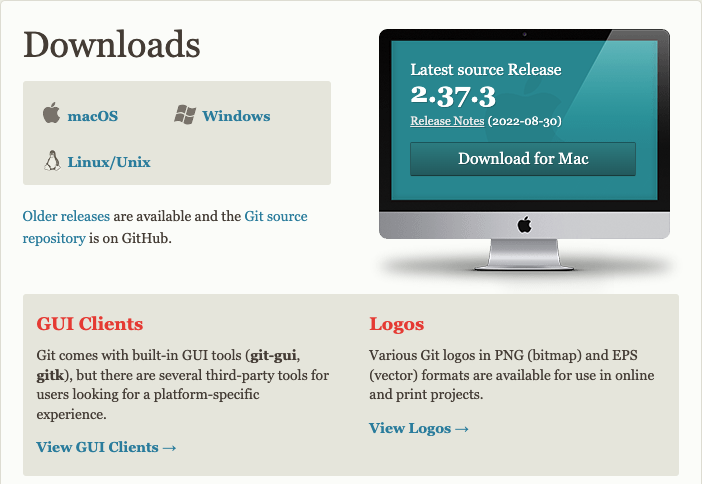
\includegraphics[scale=0.4]{Imagenes/git_01.png}
\end{figure}

Dependiendo del sistema operativo tendremos que seguir las correspondientes instrucciones y seguir los pasos de instalación.

\subsection*{Versión para macOs.}

\begin{figure}[H]
    \centering
    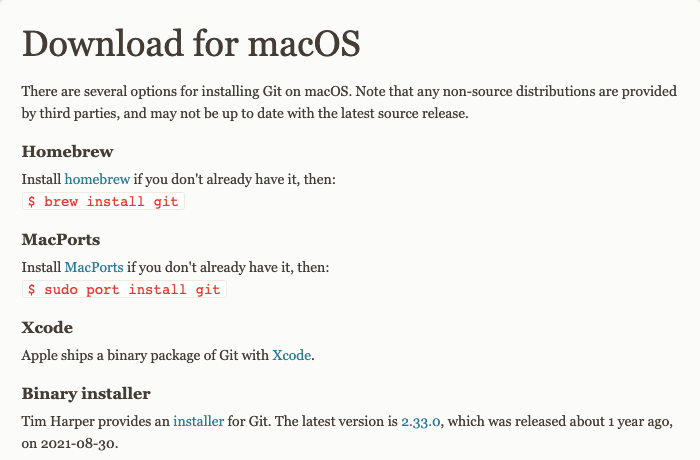
\includegraphics[scale=0.35]{Imagenes/git_02.png}
\end{figure}

\subsection*{Versión para Windows.}

\begin{figure}[H]
    \centering
    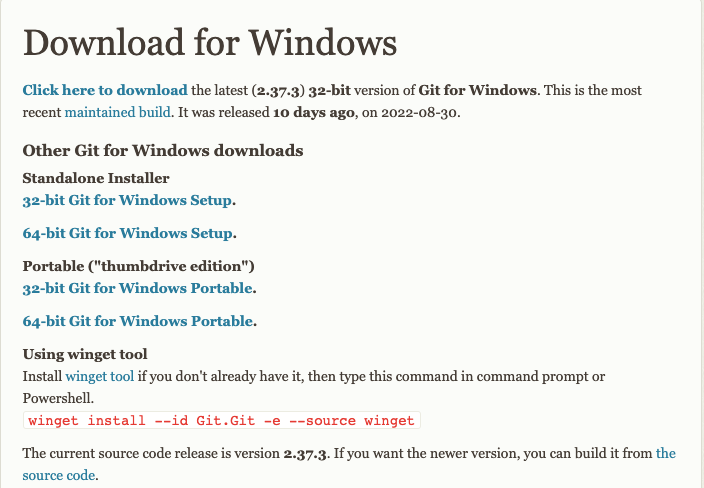
\includegraphics[scale=0.35]{Imagenes/git_03.png}
\end{figure}

\subsection*{Versión para Linux.}

\begin{figure}[H]
    \centering
    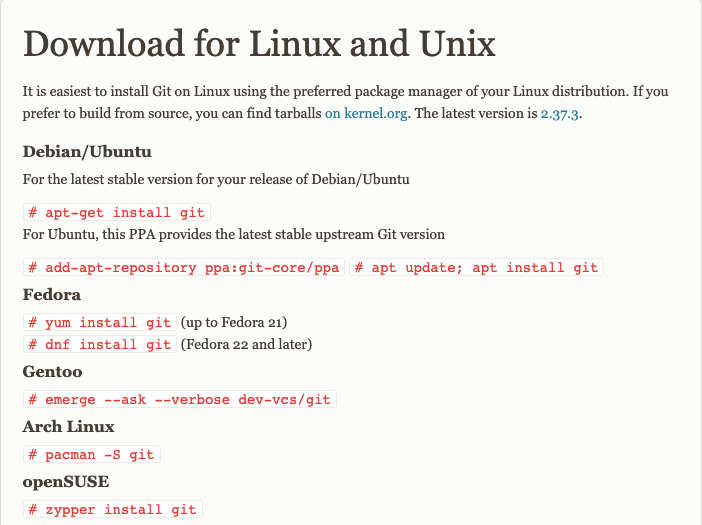
\includegraphics[scale=0.35]{Imagenes/git_04.png}
\end{figure}

Para verificar que tenemos instalado Git, basta con que en la terminal (recordemos que el prompt en la terminal es el símbolo $\$$ ) veamos la versión que tenemos en la computadora:
\begin{minted}{bash}
$ git --version
\end{minted}
Debiendo mostrarse la versión más reciente o la que está instalada.

\section{Sobre el alcance de la guía.}

Esta guía será de ayuda para \textbf{clonar} un repositorio de \texttt{\textbf{GitHub}}, que es un sitio de almacenamiento en la nube donde se almacenan nuestros archivos. Cuando clonamos un repositorio, estamos descargando todo el conjunto de archivos tal cual los ha dejado el propietario del mismo, de tal manera que podemos trabajar de manera local en nuestra computadora.
\par
El curso de Física Computacional tiene un repositorio con los materiales de trabajo: Notebooks de Jupyter, archivos de código, imágenes, etc. con los que se nos facilitará el desarrollo en cada uno de los temas del curso.
\par
Estamos desarrollando una guía más completa para manejar Git y GitHub en donde podrán revisar todo el proceso que se requiere para que ustedes creeen, administren, compartan, trabajen y mantengan actualizados sus propios respositorios, tan pronto tengamos la guía terminada, les daremos aviso para que la consulten.

\section{Clonando un repositorio existente.}

Si queremos obtener una copia de un repositorio de Git existente, por ejemplo, un proyecto al que nos gustaría contribuir, el comando que necesitamos es \texttt{git clone}.
\par
Se clona un repositorio con: \texttt{git clone [url]}. Para el repositorio de nuestro curso, hay que conocer de antemano la dirección:
\begin{figure}[H]
    \centering
    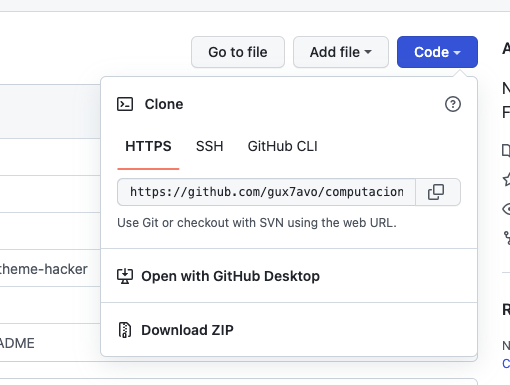
\includegraphics[scale=0.6]{Imagenes/git_05.png}
    \caption{El URL se les proporciona para que lo revisen en el navegador.}
\end{figure}

Para un manejo más cómodo, recomendamos crear una carpeta nueva y darle un nombre asociado, con una terminal nos colocamos dentro de la carpeta para escribir el comando que clonará el repositorio:
\begin{minted}{bash}
$ git clone  https://github.com/gux7avo/computacional.git
\end{minted}

Una vez realizada la clonación, ya tenemos disponible el acceso a todos los archivos del repositorio. Toma en cuenta que en el caso de los Notebooks, se pueden modificar tanto en el texto Markdown como en el código, estos cambios los va a registrar Git, pero como nos interesa solo ocupar los archivos para trabajo complementario, no será necesario enviar los cambios al repositorio. Cuando manejes tus propios repositorios, verás que es necesario contar con las credenciales de ingreso a GitHub y que desde tu cuenta, des los permisos necesarios para aceptar cambios en los archivos.
\par
Cuando el equipo académico agregue nuevos archivos al repositorio se les dará aviso para que actualicen el repositorio de manera local, ya no será necesario clonar nuevamente el mismo.

Abriendo la terminal y dentro de la carpeta donde se hizo la clonación, tecleamos el comando:
\begin{minted}{bash}
$ git pull
\end{minted}
    
De esta manera ya tenemos la última versión de todo el repositorio en nuestra computadora.

\section{Referencias para consulta.}


\renewcommand{\refname}{Libros.}

\begin{thebibliography}{9}

\bibitem{Chacon2014}
Scott Chacon and Ben Straub (2014) \emph{Git Pro}, APress, 2nd ed.
    
\bibitem{Galloway2021}
Jon Galloway (2021) \emph{Git for Programmers}, Packt Publishing.

\bibitem{Belanger2021}
Chris Berlanger (2021) \emph{Git Apprentice}, Razeware LLC.

\bibitem{Uzayr2022}
Sufyan bin Uzayr (2022) \emph{Mastering Git. A Begginer's Guide}, CRC Press.

\end{thebibliography}

\subsection*{\Large{En internet.}}

Para abrir la liga presiona \keys{\ctrl} + click izquierdo del ratón sobre el texto en color rojo.
\begin{enumerate}[label=\alph*)]
\item \href{https://git-scm.com/}{Sitio web de Git.}
\item \href{https://git-scm.com/video/what-is-version-control}{¿Qué es el control de versiones? (Video)}
\item \href{https://git-scm.com/video/what-is-git}{¿Qué es Git? (Video)}
 \end{enumerate}



\end{document}